\chapter{Background}
\label{background}

In this section we present an overview of the theoretical items necessary to our task of generating natural language from code features.
We start with an overview of language models, defining what they are, and noting where our task fits in the traditional NLP tasks of conditional langauge generation.
Then we provide an overview of the relevant representation learning techniques we use to achieve our goal.
Finally we conclude with a brief overview of the structure of source code, in particular its representation as an Abstract Syntax Tree, and set of Path-Contexts. 

% In this section we first present an overview of the theoretical items necessary to our task of generating natural language from code features.
% % In particular we cast our sequence generation problem in the commonly used framework of machine translation, exploring language models, translation techniques, and neural approaches to them. 
% In particular we explore the commonly used framework of machine translation, covering language models, translation techniques, and neural approaches to them. 
% We finally present an overview of the features of code that differentiate it from natural language, and conclude with a review of relevant work in the field.

\section{Language Modelling} % (fold)
\label{sec:lstm}

\subsection{Introduction} % (fold)
\label{sub:recurrent_neural_networks}

% In order to accurately model sequences of words, we often require an  require an evaluation of the true probability of distribution sequence of words.
Although natural language has the potential to be rich and complex, more often than not it is mundane and repetetive \citep{c._e._shannon_prediction_1951}. 
It is such repetitiveness that makes it possible to predict in many instances. For instance, in natural English the phrase ``\textit{The music is loud, turn it ...}", is much more likely to be followed by `\textit{off}', or `\textit{down}', than the word `\textit{around}'.
This is because the actual distribution of utterances is very sparse in  the vast space of possible utterances in natural language.

In our task, we seek to generate sequences of natural language, $\{y_1, y_2,..., y_n\}$ from a set of features of code, $\mathcal{C}$.
Ideally we seek to do this through maximising a probability:
\begin{align}
p(y_1, y_2,...,y_n | \mathcal{C}) \propto p(\mathcal{C} | y_1, y_2,...,y_n )  p(y_1, y_2,...,y_n )
\end{align}
where the proportionality follows from Bayes' rule.
This $p(y_1, y_2,...,y_n )$ term in this equation represents the probability of the sequence occuring naturally in the language. This term is what  language models aim to represent.

Language models are an unsupervised means of determining the natural distribution of utterences in a language or corpus. 
Often these utterences are broken down into single token sequences, and the probabilities are formed as a product of conditional probabilities.

\begin{align}
p(y_1, y_2,...,y_n ) = p(y_n | y_1, y_2,...y_{n-1} )  p(y_1, y_2,...y_{n-1} ) \\
= p(y_n | y_1, y_2,...y_{n-1} ) p(y_{n-1} | y_1, y_2,...y_{n-2} )...p(y_1) \nonumber\\
 = \prod_{i=1}^{n} p(y_i | y_1^{i-1} )  
\end{align}
where $y_1^{i-1} =  \{y_1, y_2,...y_{i-1}\}$ is the sequence of tokens from $1$ to $i-1$.

These probabilities can be calculated in different ways, or under different assumptions. An n-gram model assumes a Markovian conditional independence structure, where the next token is conditionally independent of all others, given the previous $n$: 
\begin{align}
 y_t \CI y_1^{t-n} \mid y^{t-1}_{t-n+1}  \\
\therefore p(y_t | y_1, y_2,..., y_{t-1} )  = p(y_t | y_{t-n}, y_{t-n+1},..., y_{t-1}  ) 
\end{align}

These models then estimate maximum likelihood probabilities from counts of occurences in corpora, and sometimes `smooth' these probabilities to overcome the sparsity of their training data \citep{Chen:1996:ESS:981863.981904}.

Other models, such as neural language models, do not make such conditional independence assumptions and use a neural network as a function approximator:
\begin{align}
p(y_1, y_2,...,y_n ) = g(y_1, y_2,...,y_n)
\end{align}

In our work, we seek a \textit{conditional} language model, which we can sample natural language given our conditioning code features $\mathcal{C}$. This conditional modelling is central to many tasks in natural language processing, which we elaborate in the next section.

\subsection{Conditional Generation of Language}

Many tasks in NLP require the generation of natural language conditioned on observations.
Three of the largest are machine translation, automatic summarization, and captioning.
In this section we briefly compare our task to these traditional fields, noting the similarities and differences with our task across each.

\paragraph{Machine Translation}
In machine translation, the objective is to generate the most likely sequence of a target language, $\{y_1, y_2,..., y_m\}$, given a sequence in an origin language  $\{x_1, x_2,..., x_n\}$. 
The translation seeks to maximise the probability:
\begin{align}
p(y_1, y_2,..., y_m| x_1, x_2,...,x_n ) \nonumber
\end{align}
% EDIT The history and context of machine translation traditionally revolves around $\{y_i\}$ and $\{x_i\}$ being in different languages with the same semantic meaning. 
Traditionally in machine translation, $\{x_1, ..., x_n\}$ and $\{y_1,..., y_m\}$ correspond to different languages with the same semantic meaning. 
In this respect our task is not a typical translation one.
However, since our models will at times attempt to generate one sequence from another, many techniques pioneered in this field are highly transferrable to our task. 
For further introductions to Machine Translation, we point the reader to \cite{trove.nla.gov.au/work/23999611,lopez_statistical_2008}.

\paragraph{Summarization}
The task of summarization aims to extract summaries or descriptions from a document.
A helpful review of the field is presented by \citet{allahyari_text_2017}.
Typically this involves extraction and/or abstraction of a document in the same modality or language.
Our task, generating descriptions about an element of code, naturally involves two different modalities - code as input, and english as output.
However, in the best case our descriptions should reflect a true and relevant summary of the argument.
Therefore, although ours is not a typical summarization task, it is sometimes framed that way in similar work \citep{iyer_summarizing_2016}.

\paragraph{Captioning}
A final task with a parallel to ours is that of captioning. 
The distinction from summarization in this case is that captioning involves generating text from differnet modalities - often captioning image, \citep{Vinyals2015ShowAT} or parts of one \citep{Karpathy2015DeepVA}.
The parallels with our code and language task are obvious here. However, it is perhaps unfair to describe documentation of code as `caption' when it aims to be a description of only the most important parts of the code, and intentionally aims for succintness.

\paragraph{}
In summary our task falls in between a number of traditional NLP tasks and consequently related work blurs the boundaries of translation, summarization and captioning. In the next section we present an overview of the relevant theoretical components for our model, indicating their provenance from their respective fields. 

\section{Representation Learning}

Given the maturity and prominence of neural networks 
% \footnote{Quote someone}
, we assume a basic familiarity with the topic, including linear and sigmoidal layers, multilayer perceptrons, the backpropagation algorithm and stochastic gradient descent. For those seeking a further background on this topic, we strongly recommend a number of books \citet{nielsenneural,Goodfellow:2016:DL:3086952}. 



\subsection{Distributed Representations} % (fold)
\label{sub:embeddings}

The vocabulary of natural language is vast and nuanced. 
Some words may appear very different lexically yet have similar semantic meaning - for instance `big' and `large'.
Others may appear lexically similar, but have different meanings - `large' and `largesse'. 
In our language generation tasks we wish to generate words that have the correct semantics.
As such it would be helpful to find numerical representations of words that reflect their semantic meaning. 

One way of doing this is to distribute the semantic meaning over various components of a vector in a high dimensional space. In this space, `big' and `large' would be closer together than `large' and `largesse'. We could then use these pretrained representations, or \textit{word vectors}, in our natural language modelling as a form of transfer learning \citep{hinton_parallel_1986}.
 % Such an idea is not new \cite{hinton_distri,buted_nodate}, but recent applications of it have become widespread in statistical NLP. 
 % REPHRASE but recent have shown trememendous benefits in training of models in recent years. CITE 

However, this begs the question: how do we etablish semantic equivalence in the first place? This is addressed the theory of distributional semantics which suggests that words which appear in similar contexts also have similar meanings \citep{harris_distributional_1954}.
To quote linguist J.R Firth : \textit{``You shall know a word by the company it keeps."} \citep{firth_synopsis_1957}

As a result, methods of training word vectors often revolve around word co-occurences.  Traditional methods of doing this involved counting co-occurences of words in a corpus, and performing matrix decomposition on the co-occurence matrix \citep{deerwester_indexing_1990}. More recently neural networks have been used to train these vectors directly, using a local context window around the word in question, with much success \citep{mikolov_efficient_2013,mikolov_distributed_2013}. An approach which combines both local window methods and matrix factorization methods is that of GloVe embeddings, by \citet{pennington_glove_2014}, which we use in our experiments. 
We make use of these embeddings to decode the words generated from our model, as their effectiveness has been demonstrated in a range of NLP tasks \citep{young_recent_2017}.




% A traditional approach to finding distributioned representations includes counting cooccurences of words in a corpus, and performing matrix decomposition on the co-occurence matrix \cite{deerwester_indexing_1990}.  This is based on a core theory of distributional semantics dating back to Harris 1954 \cite{harris_distributional_1954}, that words which appear in the similar contexts have similar meanings. To quote linguist J.R Firth in 1957: ``You shall know a word by the company it keeps.'' \cite{Firth1957}
% Other methods of capturing semantic meaning include counting occurences in local window around the word in question, and have also proved effective \cite{mikolov_efficient_2013}.

% Glove embeddings, by Pennington et al \cite{pennington_glove_2014}, combine both local window methods and matrix factorization methods to derive their distributed represetations (word vectors).  
% In our experiments we make use of pretrained GloVe pretrained embeddings to decode the words generated from our model, as similar work has demonstrated their assistance in training $<$CITE$>$.

\subsection{Recurrent Neural Networks} % (fold){}
\label{sub:recurrent_neural_networks}

% Natural language has an inherent sequential structure. The length of this sequence can stretch beyond sentences as context can change the meaning of phrases.
% Basic neural networks such multilayer perceptrons, are poorly suited to capturing sequential information, as they are unable to remember information from previous tokens in a sequence.
A recurrent neural network (RNN) is a neural network with recurrent connections between neurons. These connections allow the network to pass on information as it processes a sequence (see Figure \ref{fig:unrolled_lstm}). In effect this forms a hidden state in the network,  allows information from previous tokens to propagate inside the network and contextualise the processing of future tokens.
Such networks have proved highly adaptable to many NLP tasks \citep{young_recent_2017}, such as language modelling \citep{t._mikolov_extensions_2011} and translation \citep{liu_recursive_2014}, due to the inherent sequential nature of the structure of language. They have also enjoyed widespread use within many other sequence learning settings \citep{lipton_critical_2015} .

\begin{figure}[h]
    \centering
    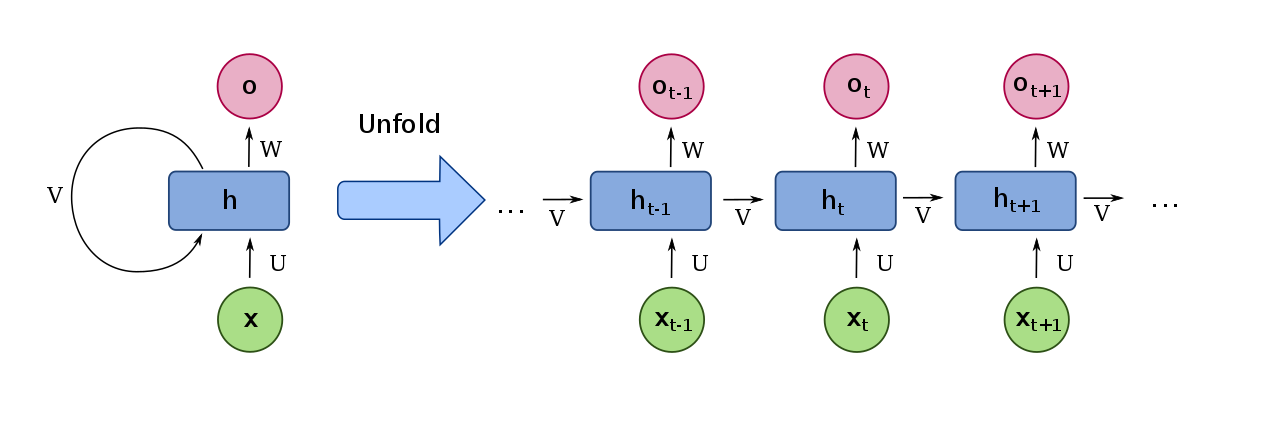
\includegraphics[width=.9\linewidth]{ModelPics/rnn_wiki.png}
    \caption{A diagram of an RNN. This demonstrates how a recurrent connection can be `unrolled' to form an effective hidden state maintained by the network as it processes as sequence.  }
    \label{fig:unrolled_lstm}
\end{figure}

% Much of the semantic meaning of language is captured in the order of words. 
% % It is not only the lexical tokens, but the sequence of them, that carries the information of a sentence.
% This order can stretch beyond sentences, as context too can change the meaning of a sentence or phrase.
% Vanilla neural networks such as multilayer perceptrons are poorly suited to capturing such long range information, as they are unable to remember preceding tokens in a sequence. 
% Furthermore, they struggle from problems of vanishing and exploding gradient when processing long sequences \cite{bengio_learning_1994}.

% A recurrent neural network (RNN) is one in which a hidden state is maintained by the network, while processing a sequence.
% This hidden state allows information from previous tokens to propagate inside the network and contextualise the processing of future tokens.
% Such networks have proved highly adaptable to language tasks, and enjoy widespread use within many sequence learning settings\cite{lipton_critical_2015}. They are also more resistant to the vanishing and exploding gradient problems.

An example of an RNN is the Long Short Term Memory Unit (LSTM) \citep{hochreiter_long_1997}. We use this RNN due to it's intrinsic ability to deal with the common training problems of vanishing and exploding gradients 
\citep{bengio_learning_1994}. These comprise of four gating mechanisms, ($\mathbf{f_t}, \mathbf{i_t},\mathbf{\tilde{c_t}}, \mathbf{o_t}$), operating on the input $\mathbf{x_t}$ and state vectors $\mathbf{c_t}$ and $\mathbf{h_t}$. 
Each gating mechanism has a corresponding weight matrix, $\mathbf{W}$, and bias vector $\mathbf{b}$, and operate according to the following equations:

\begin{align}
    \mathbf{f_t} = \sigma(\mathbf{W}_f [\mathbf{h_{t-1}}, \mathbf{x_t}] + \mathbf{b_f})\label{eq:lstm1}\\
    \mathbf{i_t} = \sigma(\mathbf{W}_i [\mathbf{h_{t-1}}, \mathbf{x_t}] + \mathbf{b_i}) \label{eq:lstm2}\\
    \mathbf{o_t} = \sigma(\mathbf{W}_o [\mathbf{h_{t-1}}, \mathbf{x_t}] + \mathbf{b_o}) \label{eq:lstm3}\\
    \mathbf{\tilde{c_t}} = \tanh(\mathbf{W}_c [\mathbf{h_{t-1}}, \mathbf{x_t}] + \mathbf{b_c}) \label{eq:lstm4}
\end{align}
where [,] operator indicates concatenation and $\sigma$ indicates element-wise sigmoidal function.

These gating equations then combine to update the cell state $\mathbf{c_{t-1}}$ and the hidden state $\mathbf{h_{t-1}}$ as follows: 
\begin{align}
    \mathbf{c_t} = \mathbf{f_t} * \mathbf{c_{t-1}} + \mathbf{i_t} * \mathbf{\tilde{c_t}} \label{eq:lstm5}\\
    \mathbf{h_t} = \mathbf{o_t} * \tanh(\mathbf{c_t}) \label{eq:lstm6}
\end{align}

where  $*$ indicates element-wise multiplication, and tanh indicates element-wise hyperbolic tan.

Interpretting these operations gives a good insight into the success of the LSTM.  
Equation \ref{eq:lstm1} represents the creation of a `forget' gate, where vector $\mathbf{f_t}$ represents what fraction of each dimension of $\mathbf{c_{t-1}}$ to retain. 
Equation \ref{eq:lstm2}  creates an `input' gate, where vector $\mathbf{i_t}$ represents what fraction of each dimension of our transformed input $\mathbf{\tilde{c_{t}}}$ we want to retain.  
$\mathbf{\tilde{c_{t}}}$ itself is created in equation \ref{eq:lstm4}. With both the `input' and `forget' gate, the  the cell state is updated in \ref{eq:lstm5}. 
The new hidden state $\mathbf{h_{t}}$ then derives from this cell state, which is modified by the output gate $\mathbf{o_t}$. 
Both $\mathbf{c_{t}}$ and $\mathbf{h_{t}}$ pass forward to the next time step, while $\mathbf{h_{t}}$ is also out put by the cell. 
A diagram is presented in Figure \ref{fig:lstm_colah}.

\begin{figure}[tb]
    \centering
    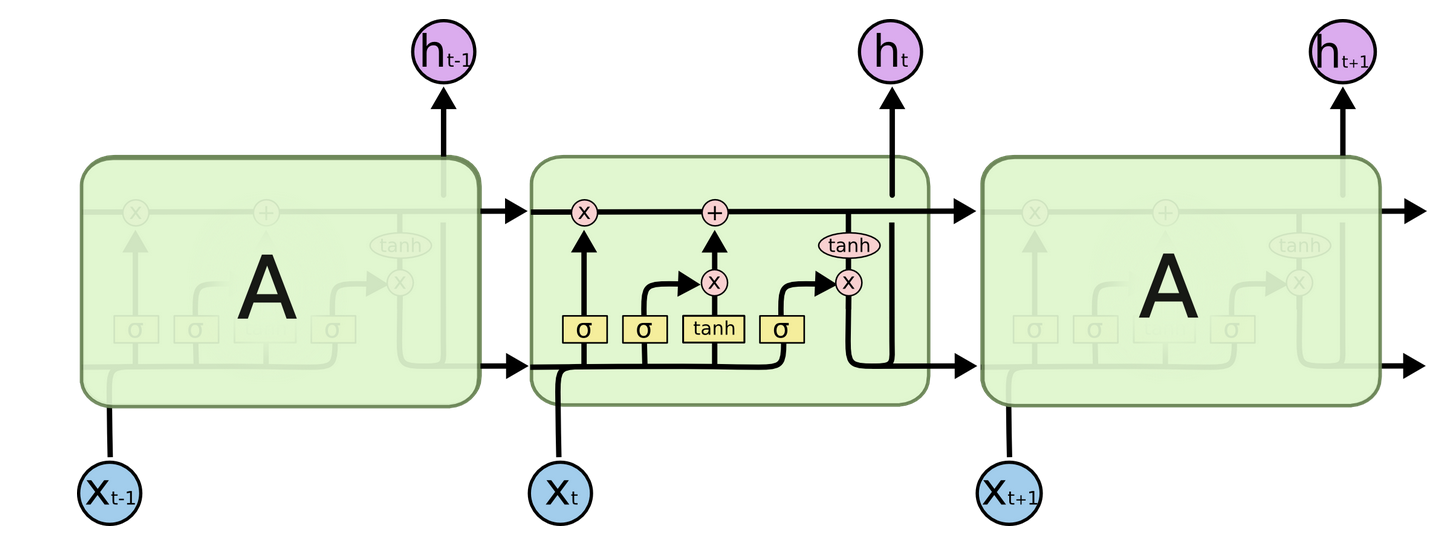
\includegraphics[width=\linewidth]{ModelPics/LSTMcolah.png}
    \caption{A diagram of an LSTM, sourced from \cite{noauthor_understanding_nodate}}
    \label{fig:lstm_colah}{}
\end{figure}

LSTM's have shown a remarkable versatility and strength in NLP tasks \citep{young_recent_2017}. In fact, a remarkable study of language modelling in 2017 showed that well-tuned LSTMs still surpass more recent and complex architectures, and achieve state of the art results, despite their relative simplicity \citep{melis_state_2017}.

There also exist other forms of RNN units. The Gated Recurrent Unit \citep{cho_properties_2014}, is another recurrent network unit that aims to simplify the LSTM, and has shown comparable performance to the LSTM in tasks such as speech signal modelling and music modelling \citep{chung_empirical_2014}.
However, for the purposes of our investigation, we use the LSTM for all recurrent units.

%BIDIRECTIONAL LSTMS??

\subsection{Sequence-to-Sequence Architectures} % (fold)
\label{sub:sequence_to_sequence_architectures}

At each time step, an RNN unit accepts an input $\mathbf{x_t}$ and emits an output $\mathbf{h_t}$. In the translation context, this 1-to-1 mapping of input to output is the equivalent of translating a sentence before you hear the end of it. For languages such as German, where the verb comes at the end of the sentence, this presents a big challenge.

\begin{figure}[tb]
    \centering
    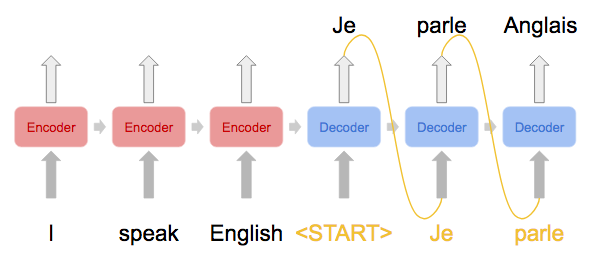
\includegraphics[width=\linewidth]{ModelPics/seq2seq.png}
    \caption{An example of sequence to sequence architecture}
    \label{fig:seqtoseq}
\end{figure}

The sequence-to-sequence (Seq2Seq) architecture, originally proposed by \citet{sutskever_sequence_2014}, overcomes this limitation by processing the whole input sequence before translation even begins. 
In this framework, presented in Figure \ref{fig:seqtoseq}, an RNN acts as encoder, through which all word tokens are passed. 
It acts as an encoder because its final hidden state is taken to be an encoding of the sequence into a intermediate representation. 
This representation is then used as the initial state of a decoder rnn cell, to conditionally generates a sequence of tokens.

First a ``start-of-sentence" token is fed into the decoder, generating a distribution over tokens, conditioned on the initial state from the encoded vector. 
Then most likely token is chosen, and fed back into the decoder, generating a distribution over the next one. 
This method repeats until the sequence terminates, perhaps with a ``end-of-sentence'' token.

This describes a greedy form of decoding, where the most likely next word is continually selected from the decoder.  It is also possible to explore the broader space of translations, by feeding in multiple tokens and retaining only the most likely sequences. This technique is known as beam search \citep{freitag_beam_2017-2}.

This architecture, though effective, has some drawbacks. It has been shown that as the source sequence gets longer, the performance of the model worsens significantly \citep{cho_properties_2014}. 
This is partly due to the fact that model must now compress more information into the intermediate vector passed between encoder and decoder. A common way of dealing with such an issue is to use attention. 

% What are the problems: long sequences
% Forgetful of what happens at the beginning - bi rnns
% Application to machine translation. 
% Raw code tokens to language - limited success



\subsection{Attention} % (fold)

\begin{figure}[tb]{}
    \centering

    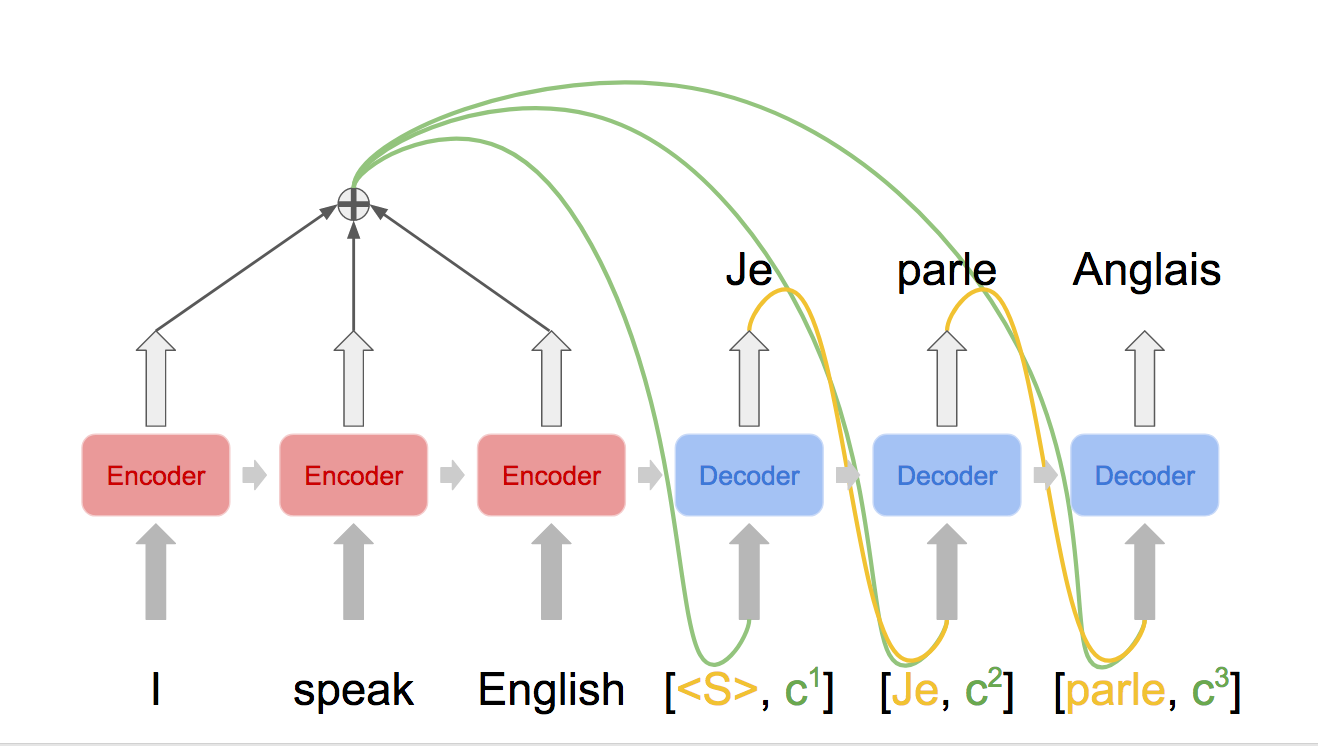
\includegraphics[width=.7\linewidth]{ModelPics/bahd_diag.png}
    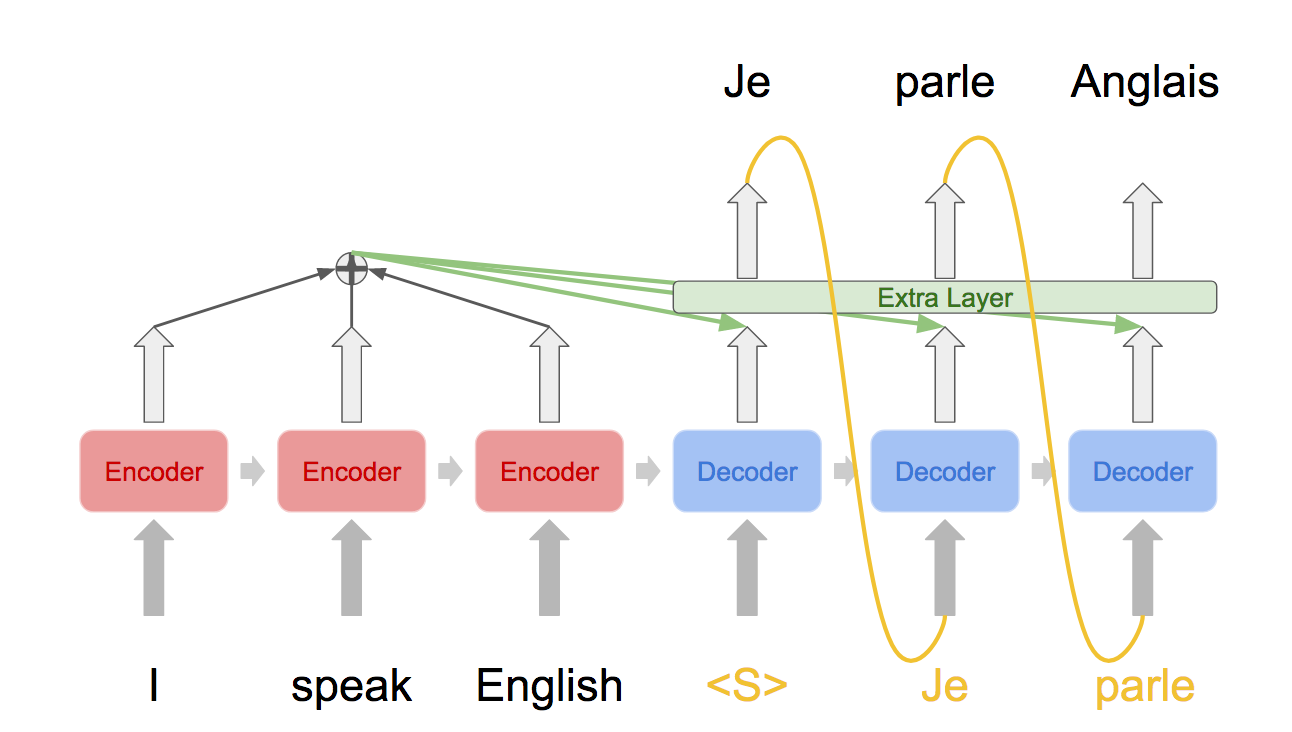
\includegraphics[width=.7\linewidth]{ModelPics/luong_diag2.png}
    \caption{Two example of sequence to sequence architecture with attentional models: Badanau Attention (above), Luong Attention(below)}
    \label{fig:attention} 
    % \label{fig:luongattention}
    % \caption{An example of sequence to sequence architecture with Badanau attention}

\end{figure}


As the sequences get longer, encoder-decoder architectures struggle to pass the full information required from the encoder to the decoder. 
One way of improving this is to augment the decoding process with a contextual vector at each step.  
As before, the decoder estimates the conditional probability for the next word $y_t$, given the input sentence $\mathbf{x}$, and previous output tokens ${y_1, ..., y_{t-1}}$.
 However, this changes from being a function of simply the input token, $y_{t-1}$, and hidden state, $s_{t}$ at step $t$:
\begin{equation}
p(y_t| y_1, ..., y_{t-1}, \mathbf{x} ) = g(y_{t-1}, s_t)
\end{equation}
to now being a function of the context vector at that point $c_t$ aswell:
\begin{equation}
p(y_t| y_1, ..., y_{t-1}, \mathbf{x} ) = g(y_{t-1}, s_t, c_t)
\end{equation}

The context vector at each step is itself calculated using a weighted sum of the RNN outputs $\{h_1,... h_{t_1}\}$:
\begin{equation}
c_t = \sum_{j=1}^{T_x}\alpha_{tj}h_j
\end{equation}
where
\begin{equation}
\alpha_{tj} = \dfrac{\text{exp}(a(s_{t-1}, h_j))}{\sum_k^{T_x}\text{exp}(a(s_{t-1}, h_k))}
\end{equation}
and $a$ is a function that maps to the reals - often a multilayer perceptron that is trained simultaneous to main training. 

This method was introduced by \citet{bahdanau_neural_2014} who demonstrated that the networks could use the attention to align words during translation.
In this case the $\alpha$ parameter acts like a weighting indicating the most important word used in each token generation - which word the decoder should pay attention to.

Variations on attention (as demonstrated in Figure \ref{fig:attention})) have found great use in the field of machine translation  \citep{luong_effective_2015}, and have even demonstrated their use independently of RNNs in this field \citep{vaswani_attention_2017}.  They have also have demonstrated their effectiveness in fields such as captioning, where they prove an effectve way of working with different modalities \citep{xu_show_2015}.

In our models we use attention mechanisms extensively, both as a means of dealing with particularly long sequences (in our case of characters), and also as a means of dealing with the difficult modality of code.




\section{Structure of Code} % (fold)
\label{sec:translating_code}

Although in principle the models presented in this thesis could be applied to any programming language, our dataset consists of functions in the Python prgramming language.  
In this section we provide a brief introduction to the language before presenting a broader overview of abstract syntax trees.

\subsection{Introduction to Python} % (fold)
\label{sub:python}

Python is a \textit{dynamically-typed} language, meaning that the `type' of an object, such as `string' or `integer', is be decided at runtime, rather than specified in advance, or \textit{statically}.
This allows a greater flexibility in the language, but comes at the expense of a less informative source code.
Declaring a variable \mintinline[]{python}{var}, makes no guarantees on what it could be, or how it can be used. 

Furthermore Python is \textit{strongly-typed} language, meaning that a type can not be implicitly coerced into another one by the computer at run time. Changes in type must be explicit. For instance, evaluating \mintinline[]{python}{1 + '0'} would result in an \mintinline[]{yaml}{TypeError} being raised in Python. In \textit{weakly-typed} JavaScript this returns \mintinline[]{python}{'10'}.
This means that inappropriate use of variables can lead to run time crashes or errors very easily in Python.

\begin{listing}[h!] 

\begin{minted}[fontsize=\footnotesize]{python}
def xkcd_palette(colors):
    """Make a palette with color names from the xkcd color survey.
    This is just a simple wrapper around the ``seaborn.xkcd_rgb`` dictionary.

    Parameters
    ----------
    colors : 
        List of keys in the ``seaborn.xkcd_rgb`` dictionary.

    Returns
    -------
    palette : 
        Returns the list of colors as RGB tuples in an object that behaves like
        other seaborn color palettes
    """
    palette = [xkcd_rgb[name] for name in colors]
    return color_palette(palette, len(palette))

\end{minted}

    \caption{A source code snipped from the validation set, with  a numpy-style doctring. The docstring presented been trimmed for brevity.}
    \label{fig:docstring}
\end{listing}




Together, these features make documentation an especially important part of Python. 
Functions and classes therefore have a built-in convention for containing documentation, called a docstring. 
This is automatically displayed when the built-in \mintinline[]{python}{help} is called on the function.
A typical function with a docstring is illustrated in Figure \ref{fig:docstring}. 
Many open source libraries document their API's with HTML built straight from the docstring of the underlying methods.

There are no explicit rules for how docstrings must be written, but two popular conventions are those the Google\footnote{https://sphinxcontrib-napoleon.readthedocs.io/en/latest/example\_google.html\#example-google} and numpy\footnote{https://sphinxcontrib-napoleon.readthedocs.io/en/latest/example\_numpy.html\#example-numpy} conventions. These specify that the arguments of a function explicitly be described in the docstring, along with the description of the function.
Our project involves sourcing and parsing functions that use these conventions, to be able to get the close mapping between the elements of the source code (the arguments) and their human written descriptions. 


\subsection{Abstract Syntax Trees} % (fold)
\label{sub:abstract_syntax_trees}

Programming languages communicate along two channels \citep{allamanis_survey_2017}. The \textit{human readable channel} consists of the lexical names and words in files as read and written by humans.  The \textit{computer readable channel} consists of the information that forms the direct instruction set aimed at the computer.
This direct instruction set is stripped of information superfluous to computer, such as comments and names, and is therefore difficult for humans to interpret directly.
The instruction set is also represented by an intermediate structure, known as an abstract syntax tree (AST).
This is directly obtained by parsing the written source code, and wholly specifies the instructional information to the computer.
It is therefore the perfect data structure to investigate patterns in the computer readable channel.

The form of ASTs differ from language to language. 
Each language may have a different set of nodes and variables, and information associated with them.
However, in general an algorithm that operates on one AST should be transferrable to another. 



\begin{figure}[tb]

    \centering
    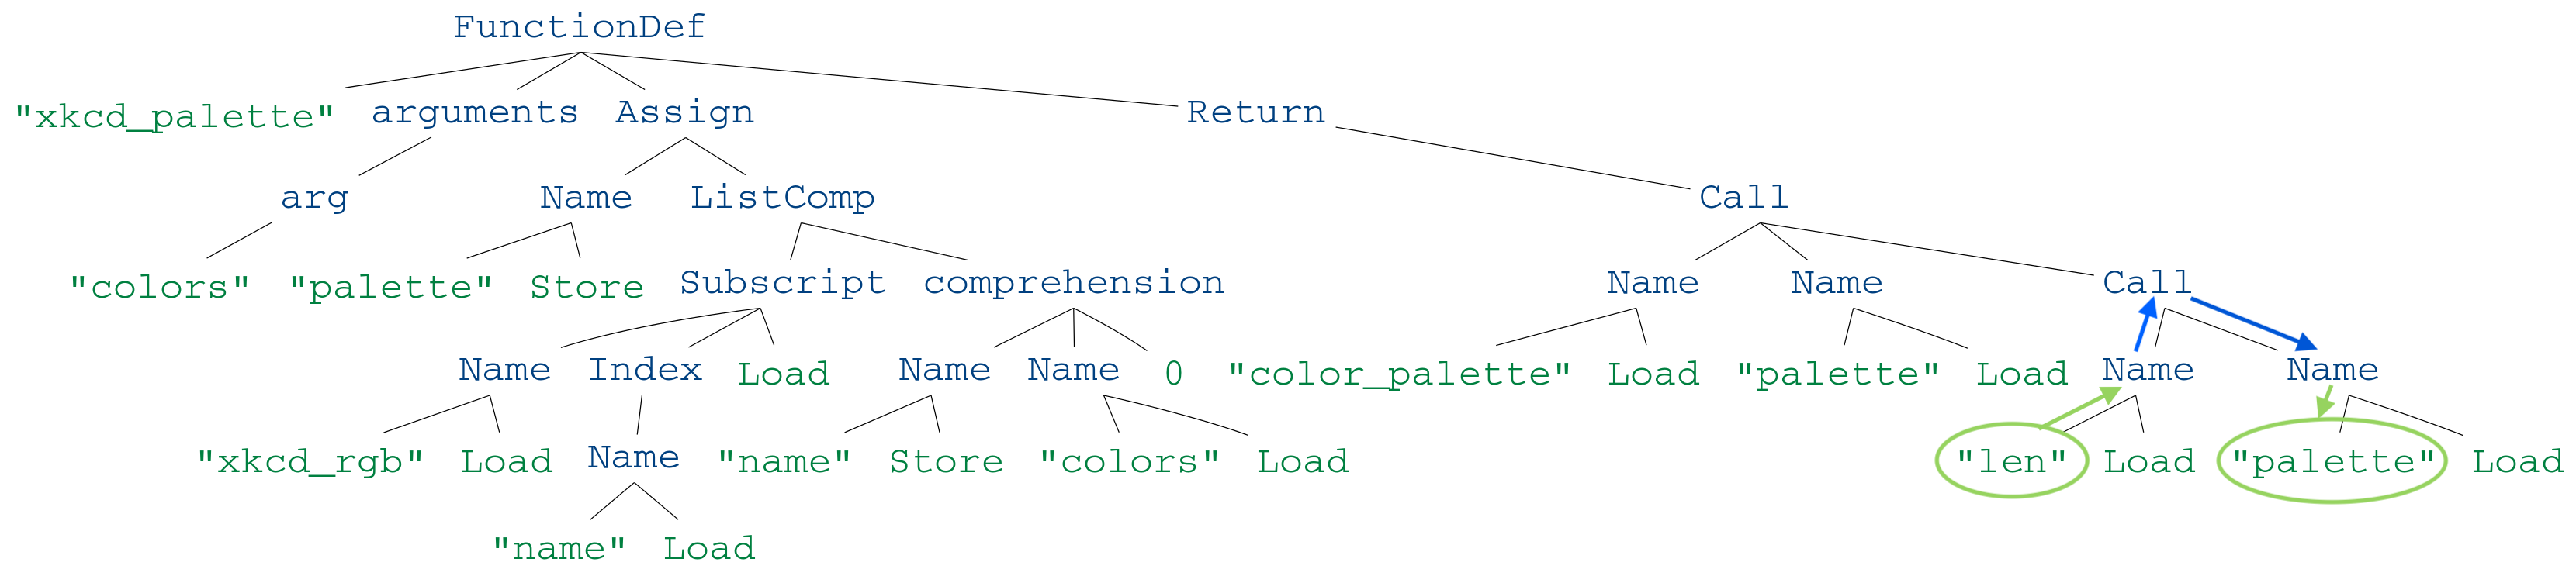
\includegraphics[width=\linewidth]{ModelPics/xkcd_palette_strip_full_copy.png}
    \caption{The Python AST corresponding to the code in Figure \ref{fig:docstring}. We omit the node containing the docstring for clarity. Terminal nodes are shown in green, non-terminal nodes are shown in blue. We highlight a path from \mintinline[]{yaml}{"len"} to  \mintinline[]{yaml}{"palette"}}
    \label{fig:fullAST}

(\mintinline[]{yaml}{"len"}, string $\uparrow$ Name $\uparrow$ Call $\downarrow$ Name $\downarrow$ string ,  \mintinline[]{yaml}{"palette"})
    \caption{An example of a \textit{path-context}, from the highlighted path in the above AST.}
    \label{fig:path_eg}

    (Name $\uparrow$ Call $\downarrow$ Name,  \mintinline[]{yaml}{"palette"})
    \caption{Example \ref{fig:path_eg} as a \textit{variable path-context} for the variable \mintinline[]{yaml}{"len"}}
    \label{fig:varpath_eg}
\end{figure}


In our project, we work with the Python AST, as visible in Figure \ref{fig:fullAST}.
This is composed of a series of instruction nodes, that terminate with lexical names. 
These names are the names of objects, which could therefore be methods, variables, classes, etc. 
In fact, in Python everything is an object.\footnote{https://jeffknupp.com/blog/2013/02/14/drastically-improve-your-python-understanding-pythons-execution-model/} 
As can be seen from the syntax tree, sometimes these object names are being loaded into memory and at other times other objects are being assigned to them.

In our project we aim to see if a statistical approach to looking at the structure or substructure of the AST can lead us to making inferences that will translate to language. 
For instance, the use of certain AST subtrees may suggest the type of an object or how its used in a function.
These kind of inferences are powerful, because they should be robust to trivial lexical changes, like renaming a variable.

\subsection{Path-Contexts and Variable Path-Contexts} % (fold)
\label{sub:abstract_syntax_trees}

Although the AST is the definitive data structure that code is parsed into, it is also possible to reparameterise the tree as a set of shortest paths between terminal nodes. 
This is the reparameterisation that \citet{alon_general_2018} developed to facilitate learning on syntax trees.

In this reparameterisation, an AST is made up of terminal nodes $\mathcal{T}$, and non-terminal nodes $\mathcal{N}$. 
A path $p$ of length $k$, represented as $n_{1}d_{1}n_{2}d_{2}...n_{k-1}d_{k-1}n_{k}$, where $n_i \in (\mathcal{N} \cup \mathcal{T})$, and $d \in \{\uparrow, \downarrow\}$. 
A \textit{path-context} is then defined as a triple $(x_s, p, x_f)$, where $x_s = val(n_1) $ and $x_s = val(n_k)$, $n_1,n_k \in \mathcal{T}$ and $val$ returns the value of the node \citep{alon_general_2018} 
An example \textit{path-context} from the furthest right of the example AST is shown in Figure \ref{fig:path_eg}.

The advantage of this representation is that it breaks down AST into a set of locally connected pieces, each involving two well-defined variables.
This setup is highly desirable for our own investigations, except that we require the obfuscation one of the variables (our test argument).
Therefore, for the purposes of this investigation we define two new context tuples: a \textit{modified path-context}, and \textit{variable path-context}.

A \textit{modified path-context} is a triple $(x_s, p', x_f)$ defined by \textit{path-context} $(x_s, p, x_f)$, where $p = n_{1}d_{1}p'd_{k-1}n_{k}$. In otherwords, the type of the leaf nodes are not included in the new path. This is done to remove redundant information, since the Python AST is so simple that the $val( )$ of the node already specifies its type.
The \textit{variable path-context} for variable $x_s$ is then defined as the double of $(p', x_f)$ for the \textit{modified path-context} from $x_s$ to $x_f$.

Although these collections of \textit{variable path-contexts} no longer specify the entirety of the tree, the ability to pluck out features of the code from the AST that only involve our particular argument will prove very useful in our investigations. 





% \section{Related Work}

% It is only through the recent development of large open source datasets and the techniques to process them, that statistical approaches to code-related tasks have been available to machine learning researchers. 
% As would be expected of any new and growing field, the range of attempted tasks is still expanding. 


% As of writing no formal attempt has been made to automatically generate natural language descriptions of individual elements of code from its source.  
% This is not surprising given how recently the field has developed, and the lack of a suitable dataset.
% However, progress has been made in the related fields of source code summarization, variable naming, documentation generation, and code language modelling. 
% These advances highlight possible approaches to statistically modelling structure of code like language.  

% In this review we summarise the current advances of these methods and how they relate to the task at hand.  We start by examining progress in the language modelling of code, then examine sequence generation tasks, such code comment prediction, code summarization or function naming. We then examine advances in the fields of representation of programs and abstract syntax trees. Finally we present an overview the existing datasets and the scope of the problems they are suitable to address, finding them lacking in our particular domain.


% % As mentioned in the Introduction, it is only through the recent development of large open source datasets that statistical approaches to code related tasks have been available to machine learning researchers. 
% % As would be expected of any new and growing field, the range of attempted tasks is still expanding. 
% % Although as of writing no formal attempt has been made to translate fine grained elements of source code into their natural language descriptions, a great deal of relevant insight has been made in the related fields of source code summarization, variable naming, documentation generation, and code language modelling. Many of these problems highlight possible approaches to modelling the patterns and structure of code as language, and can even be cast into a machine translation framework.  

% % In this review we summarise the current advances of these methods and how they relate to the task at hand.  We start by examining with the general progress in the language modelling of code, before moving on to specific tasks that can be posed as sequence generation tasks, such code comment prediction, code summarization or function naming. We subsequently examine advance in the related fields of representation of programs, before we finally examine the existing datasets, and the scope of the problems they are suitable to address. 

% \subsection{Language Models of Source Code}

% The earliest work modelling source code with natural language techniques comes from Hindle at al \cite{Hindle:2012:NS:2337223.2337322}, who used simple Kneser-Ney smoothed n-gram models of code tokens, to create language models for large-scale Java and C projects.
% With these models, Hindle was able to demonstrate that the cross-entropy of source code within projects was lower than that of large English corpora - indicating the presence of repetetive common patterns that could be leveraged for code completion, naming and summarization.
% This was consistent with findings by Gabel and Su \cite{gabel_study_2010} who examined the lines of approximately 6000 projects of code and found widespread repetition of sections of up to several lines, both within and across projects.
% Despite the simplistic Markov chain assumption implicit in the ngram model, the effectiveness of this modelling techniques, especially within projects, opened up the field of code analysis to the wider natural language processing community.

% Hindle's model, which only took into the lexical structure of code, was improved by Nguyen et al\cite{nguyen_statistical_2013}, by integrating semantic information into the n-gram model.
% Instead of training on the raw string of the token, the \textit{lexeme}, this model condensed information such as data type, scope, role (such as literal, variable, function call) into a \textit{sememe}, and trained an n-gram topic model, modelling both local context \textit{sememes} ngrams, and global trends in the code.
% This highlighted the value of taking into account the semantic information in code, as well as the lexical, in prediction tasks.

% Since then a number of different language models of code have been developed, largely finding their use in code-completion tasks. These have demonstrated the importance of factoring in the long range dependencies of code, and elements of the code beyond simple lexical structure. For instance Tu et al added a cache mechanism to improve Hindle's ngram model in capturing longer range dependencies  \cite{tu_localness_nodate}, while this itself was surpassed (up to 9 grams) with a recurrent neural language model by White et al\cite{white_toward_2015}.
% Most recently, Bhoopchand et al used a sparse pointer network to create a language model that significantly outperformed a LSTM baseline on code completion tasks, that was able to refer to objects in code over 60 tokens previous\cite{bhoopchand_learning_2016}.

% This work in language modelling has direct applicability to our task at hand, as it points out relevant strategies in picking out the statistically important features of `natural' code. In particular we note the importance of capturing long range dependencies (as seen in neural models), with the performance benefit that can be brought by taking into account semantic information (from the instructions given to the computer).

% \subsection{Sequence Generation from Code}

% A long running task is that of code summarization. 
% This task involves taking large sections of code blocks, and summarising its meaning in natural language. It has historically had parallels with the long running (inverse) problem of semantic parsing. CITE
% As such, early approaches to this problem completely ignored the `naturalness' properties of code and its comments, and instead was tackled with rule-based methods. 

% Work by Sridhara et al \cite{sridhara_[not_2010}  used static analysis to find important semantic subunits of code in Java projects, and used sets of sentence templates to produce English from these subunits.
% % This model revolved around automatic rule-based summarization of the source code in the source code in consideration.
% This work produced text that describe the functions in question to a high degree of accuracy, but Sridhara noted the potential lack of transferrability to other settings, and lack of examples with which to compare their summaries.  
% This procedure was also inherently inflexible, relying on human crafted templates, and specified rules. Furthermore the size of the dataset, four projects in total, indicated a potential problem in the generalisability of the work to other domains, projects or even languages.

% However, the advent of the statistical approaches to code language modelling led by Hindle et al \cite{Hindle:2012:NS:2337223.2337322} signalled the start of similar approaches to sequence generation. The earliest is Movshovitz-Attias et al \cite{movshovitz-attias_natural_nodate}, who used both ngrams and topic models such as LDA to predict comments from JAVA source code. In this they found that modelling the lexical components of source code as coming from a mixture of topics - "code" and "text" - outperformed models that ignored this distinction.  This pointed to the strength of taking into account features of code (such as distinguishing comments from commands), even if such destinction were still purely on the lexical level.

% % Since then, statistical approaches have become more popular in attacking the problem, often involving much larger corpora of training data.
% % Iyer et al \cite{iyer_summarizing_2016} sourced a large dataset of code snippets and questions from Stack Overflow, a popular programming website, to attempt this problem statistically.
% Since then neural models have become popular methods of attacking sequence generation, as they capture long range dependencies in sequences, and have shown great promise in other neural translation tasks.

% A particularly successful example is that of Iyer et al \cite{iyer_summarizing_2016}, who applied a neural attentional model to the problem of generating code `summaries'. This model trainied on a large collection of snippets and questions from Stack Overflow, a programming help website.   Iyer's model combined two features: a distributed representation of the code, generated by an attentional mechanism \cite{luong_effective_2015} over code token embeddings; and an LSTM unit \cite{hochreiter_long_1997} to encode natural language tokens. Together these generated descriptions as a sequence of conditional distributions, in an encoder-decoder model. 

% As usual, this model calculated the probability of generating a length $l$
% descriptive sequence $\{y_1,...,y_l\}$ through a product of conditional probabilities of the previous $l-1$ tokens:

% $$P(y_1,...,y_l| \mathcal{C}) = \prod_{i=1}^lp(y_i | y_1, ..., y_{i-1}, \mathcal{C} ) $$

% In this case, each conditional probability was proportional to a non-linear transformation of the combination of hidden state of the LSTM $\mathbf{h_i}$ and the attentional vector  $\mathbf{t_i}$ at that point in the sequence: 

% $$\text p(y_i | y_1, ..., y_{i-1},\mathcal{C} ) = g(\mathbf{h_i}, \mathbf{t_i}) $$
% $$g(\mathbf{h_i}, \mathbf{t_i})  \propto \mathbf{W}\text{tanh}(\mathbf{W_1h_i} + \mathbf{W_2t_i})$$

% where $\mathbf{W} \in \mathbb{R}^{|N|\text{x} H}, \mathbf{W_1}$ and $\mathbf{W_2} \in \mathbb{R}^{H \text{x} H}$  and $ H$ is embedding dimensionality of words, $ N $ the vocabulary.\cite{iyer_summarizing_2016}
% A visual schematic of the model is preseted in Figure \ref{fig:Iyer}.

% Iyer et al then ran a beam search over the decoder to explore the space of likely sequences, and evaluated their generations using the BLEU-4 and METEOR metrics.

% Iyer's model achieved a new record in the performance of the code summarization task. 
% It outperformed rival NLP models such as MOSES, a phrase-based translation model \textbf{CITE \& paraphrase}, and SUM-NN, another attention based summarization model using dense layers instead of LSTMs. 
% It also achieved a first in learning to generate original sentences from arbitrary code sections, and has proved successful in other domains.  

% Loyola et al \cite{loyola_neural_2017}, for instance, adapted a similar attention model to Iyers to generate short descriptions of differnces in code.
% This time intead of training on a single piece of source code and questions, data was sourced to present pairs of code changes (`diffs') with comments describing the change (`commit messages'). 
% In this setting, the attentional model was able to generate faesible messages, both within projects and between projects.

% These attention models show the effectiveness of being able to pickout relevant portions of code at different points in sequence generation, but fail to take into account the longer term correlations of the tokens in source code. In fact by only processing source code with this kind of attention, both models treat the source code as little more than bag of token embeddings.

% In this regard, an improvement on these attentional models is that of Alamanis et al \cite{allamanis_convolutional_2016}, which uses a convolutional attention network over tokens, for the task of predicting the names of functions given their body. This is cast as `extreme summarization'.
% %aiming to capture long range correlations in code through spatial convolutions instead of temporal hidden state.

% In this model source code is split lexically into a padded sequence of embedded tokens, over which a one-dimensional convolution of fixed-width is run, creating a number of attentional feature vectors $\mathbf{\{v_k\}}$.
% These feature vectors are then element-wise multiplicatied with the hidden state of an rnn, $\mathbf{h_{t-1}}$, to be effectively `selected' for their relevance to next generated token. They are then normalised.

% This set of feature vectors is then convolved with an attention kernel, to give a set of attention weights, each corresponding to a token embedding. 
% A final attention vector $\mathbf{\alpha}$ is constructed from the convex combination of the token embeddings under the attention weights, and this vector is used to generate a distribution over the next function subtoken.
% An illustration of the algorithm with pseudo code is presented in Figure X.

% The authors of this model apply it to both the narrow task of generating function names, and that of code retrieval. In it they find that taking into account the long range features of the code in the convolutional model surpasses a baseline attentional model of the machine translation model originated by Bahdenau \cite{bahdanau_neural_2014}, and found that this performance was further improved by adding a cacheing mechanism to the model.

% Both these attention models show the strengths that attention can provide in combining the modalities of text and code. However, a key failing of both models remains their lack of appreciation for the syntax and semantics of the underlying code.
% Although Allamanis et al's model is more aware of the structure of lexical code tokens than Iyer et als, both models continue to ignore a fundamental channel of information communication through code - that of communication from human to computer.

% % Other forms of machine translation? 
% % Phrase based translation, 
% % neural mthods, 
% % pseudo code

% As of writing no published work has been applied to generating documentation of source code using the syntactical structure of source code.  However, a number of pieces of work have recently started to examine such structure in other tasks. These are the topics of the next section of review.

% \subsection{Syntactic Representations of Code}

% A number of probablistic models have attempted to capture the the syntax of code, outside of the field of documentation generation.
% Raychev et al \cite{raychev_probabilistic_nodate} use decision trees to develop the probabilistic model of code from the syntax tree, in a code-completion setting. 
% Maddison and Tarlow \cite{maddison_structured_2014} use probabilistic context free grammars to model the AST, for a generative model. 
% Neither of these approaches provides us with the natural structure we can easily use for sequence generation. 

% Allamanis et al models the AST as explicitly as a graph, adding extra edges such as "guarded by", or "last lexical use", to capture additional semantic information\cite{allamanis_learning_2017}. These graphs are then processed with a Gated Graph Neural Network in a variable naming and variable misuse classification task. 
% This last method proves remarkably effective, though it appears highly complex to implement, the additional semantic annotations added can appear particularly arbitrary. As a result of both of these, we avoid using these representations as inputs for our task.

% A simpler way to capture the syntax of the code is to reparameterise the AST.
% Since a tree can be fully specified by the set of shortest paths between all leaf nodes, an AST can now be treated as bag of these paths. This was the parameterisation was proposed by Alon et al in 2018 \cite{alon_general_2018}, and has since been applied successfully in a function name classification context\cite{alon_code2vec_2018}.

% In this model, codepaths are parameterised into `path-contexts' - triples of the two terminal node names and the specific paths connecting them.
% Each path and terminal node has a respective embedding (learnt alongside the main task), and for each path-context, the repective two terminals and path are concatenated and fed through a neural-network layer to combine into a single path-context vector.
% A general code vector is then produced from a simple attention mechanism over the every path-context vector in the tree. 


% Alon et al are able to demonstrate a performance in a function name classification task that surpasses both Allamanis et als' \cite{allamanis_convolutional_2016} and Iyer et als \cite{iyer_summarizing_2016}. This simplicity and proven effectiveness demonstrate an appealing approach to capturing semantics within the structure of with AST.

% \section{Existing Datasets}
% \label{sec:existing_datasets}

% The scope of the tasks available to challenge researchers is naturally limited by the set of available datasets.
% % Given the relative novelty of the field, there still a limitation in the number of datasets that have been collected, cleaned and are suitable for certain tasks.
% In this section we outline the current state of the available datasets for researchers looking to generate sequences from source code. In doing so we indicate why none so far is suitable our task of generating documentation or summaries from fine-grained elements of source code.

% \subsection{Stack Overflow Dataset}

% A commonly used dataset for code captioning and summarization tasks is sourced from a large corpus of questions and code snippets from the programming help website Stack Overflow, as generated by Iyer et al\cite{iyer_summarizing_2016}. In it, questions such as ``how do I concatenate entire result sets in mysql? ' are paired with the snippets of C\# or SQL which are responses to the question, posted by other users online.
% Although widely used, this dataset suffers from a number for undesirable features for our task. 

% First of all the preparation of such a dataset demonstrates a lot of arbitrary cleaning.
% Since many of the responses from the website are invalid or do not quote code, the snippets in question have been found by searching for html \mintinline[]{python}{<code>} tags in the upvoted answers. 
% The authors note that these sections of code often bore no real relevance to the question at hand. Therefore the authors were forced to train a semi-supervised classifier to filter only relevant snippets to the question at hand.
% This convoluted pipeline runs the risk of increasing the number anomalous datapoints in the dataset, whilst reducing almost a million (query,snippet) pairs from each language, down to 66,000 pairs  of C\# and 32,000 pairs of SQL.

% Furthermore, the authors noted that often the informal code snippets often contained syntactic errors, with only 12\% of SQL snippets parsing without syntactic error. They progress with a best-effort parse, but this
%  lack of code quality, naturally poses a problem for our fine grained analysis of code segments, or indeed any analysis using the syntactical properties of code.

% Finally the dataset itself lacks a lot of the context and information needed for the granular analysis necessary for individual sections of code. Not only is the natural language not tailored to specific parts of the code, but the artificial snippets lack a lot of the context of real `natural' codebases. In fact, given the snippets' only relevant context is that of the question, the authors are forced to mask items like string literals and the like, to prevent the close context of the question and nothing else. This modification of the code is also undesirable.

% Naturally in our search for an appropriate code base, we seek larger bigger elements of `real' (and fully parsing) code, with appropriate descriptions of elements, and a greater sense of `naturalness'.

% \subsection{Edinburgh Corpus}

% A recent corpus specifically tailored to code-to-text generation, is one of Python code as released by Barone and Senrich \cite{barone_parallel_2017}, which we refer to as the Edinburgh Corpus. 
% This is a set of 109,000 triplets of function declarations, bodies, and documentation strings (docstrings), scraped from the most popular projects in GitHub, using the same methodology as Bhoopchand et al. 

% In this dataset, the authors focus on finding real world code, and extracting the string, written by code authors, providing a description of each function.
% Although these source code sections and natural language strings are more `natural' than their Stack Overflow counterparts, they still don't suit our needs, mainly in the form of the language they provide. 

% The Python language enforces no constraints on the content or format of the a class or function docstring.
% As a result, unless they follow the conventions laid out by numpy or Google, authors are not required to document arguments with a specific description, or even at all.
% Instead the docstring (if it exists) will likely just present an overall view of the function, with very little reference to the inner workings or details of the code. 
% Without a section describing either arguments or specific elements in the code with their own natural language descriptions, it is impossible for us to attempt our close comparison task.
% % Sometimes the arguments 


% % This follows from principles of keeping abstraction and implementations separate -  as a black box.
% % In fact from a code-readers perspective (instead of a code-users perspective), the most informative section of the docstring is where the arguments are described. 
% % Such a segment is not always present, but if so, would be perfect for our fine grained summarization task, as it links direct elements used in the code, to their natural-language descriptions. 

% The major failing of the Edinburgh corpus is that it does not contain enough of such sections, and where they do, they are difficult to extract from the rest of the docstring as a whole.
% As such this makes the Edinburgh corpus limited to our needs.


% \subsection{Other Datasets}
% A range of other datasets also exist in the code modelling field, often with specific tasks in mind. These are often utterly unsuitable from a natural language perspective.

% For instance, a prominent corpus of data is the GitHub Java Corpus, by Allamanis and Sutton\cite{allamanis_mining_2013}. This corpus is composed of 14,800 open source Java projects, with over 350 million lines of code (LOC), and is approximately two orders of magnitude larger than the original dataset of Hindle et al. This dataset is rich and suited to its task of language modelling, but is of little use for natural language problems, given how poorly documented much open source code is.

% Similarly Bhoopchand et al's \cite{bhoopchand_learning_2016} dataset focuses on high quality code, by pulling large sections of Python from projects with more than 100 stars from GitHub, collecting 40 million LOC. 
% Despite the quality and scale of this corpus, again the lack of appropriate documentation surrounding the code makes it unsuitable to our generation tasks, let alone anything as fine-grained as we would wish.

% As a final example, Oda et al\cite{oda_learning_nodate} source a particularly interesting dataset of individual lines of Python code from the Django open source project, with a corresponding line of human-written pseudocode. Although such datasets present interesting opportunities to look at close relations between code and language, the pseudo-code is far too close to actual code to help us in this task, and is highly artificial. 



% % These attentional style models have shown great success at combining the different modalities of text and code, and this particular model
% \begin{figure}[tb]
%     \centering
%     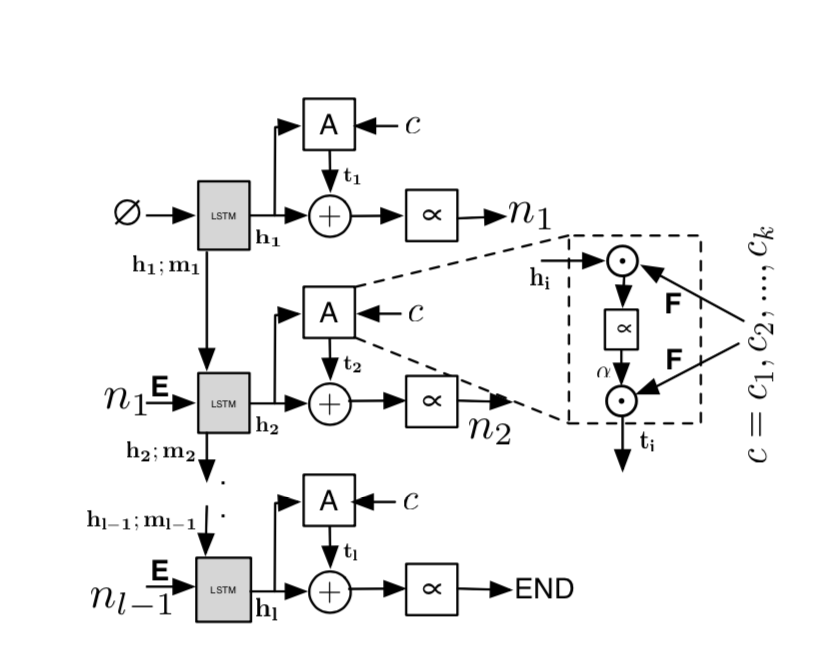
\includegraphics[width=0.5\linewidth]{ModelPics/Iyer_etal.png}
%     \caption{Iyer et als Code NN, taken from \cite{iyer_summarizing_2016}}
%     \label{fig:Iyer}
% \end{figure}



